\section{Numerical experiments in the mean-field limit}

\label{2302:sec:app:numerics-mean-field}
In this appendix we show the result of some numerical experiments we performed to verify the statements exposed in Section~\ref{2302:sec:meanfield}.  We also refer to our \href{https://github.com/IdePHICS/DimensionlessDynamicsSGD}{GitHub repository}.  

First, we checked that the point \(\Q^\bot = 0\) is a fixed point of the dynamic.
We compare a simulation of this case with an integration of just the matrix \(\M\). Since when \(\Q^\bot = 0\), \(\M\) is a \emph{sufficient statistic} by itself, we expect it to be the only parameter to be evolved to characterize the dynamics.
Figure~\ref{2302:fig:mf-numerical-simulation-appendix}~(a) shows agreement between simulation and ODE integration. 

Secondary, we would like to test is the actual need to calculate expected value on the matrix \(\Xi\) when integrating the mean field in low dimension.
In Figure~\ref{2302:fig:mf-numerical-simulation-appendix}~(b) we present the results for \(\erf\) activation function: not taking into account the off-diagonal terms, the integration of the ODEs do not match the simulated dynamics even for large \(\hids\). 
The effect becomes even more evident by comparing  Figure~\ref{2302:fig:mf-numerical-simulation-appendix}~(c) with Figure~\ref{2302:fig:meanfield-limit}~(a). In fact, we can see that in the case of quadratic activation, neglecting the matrix \(\Xi\) leads to a mismatch of population risk even at the initial instant, as it follows naturally from Equation~\eqref{2302:eq:def:mf_square}.
We do not see such a marked difference in the case of \(\sigma=\erf(\sfrac{\cdot}{\sqrt2})\) since the latter is an odd function and non-diagonal terms of $\Xi$ are symmetric random variables.

Finally, we looked at the evolution of the distribution of student weights. We use $k=1$ to have just one teacher vector $\vec{w}^{\star}\in\mathbb{R}^{d}$, while \(p=5000\) to have enough samples to understand how the distribution is evolving. In particular, we are looking at the distribution of the cosines of the angles between student weights and $\vec{w}^{\star}$; in Figure~\ref{2302:fig:mf-numerical-simulation-appendix}~(d) we plot this distribution at 3 different times of the evolution.
At \(t=0\), the distribution is uniform, as expected since we sample weights from a spherical invariant distribution with \(d=3\). 
During the evolution, the student's weight moves in the direction of $\w^\star$ and $-\w^\star$ (since $\act$ is an even function the sign of the weights does not count). At large time, the distribution is essentially $\sfrac12\left(\delta_{\w^\star} + \delta_{-\w^\star}\right)$, which represents perfect learning.
%: $\sfrac{\M_{j1}}{\sqrt{\P_{11}\Q_{jj}}} = \sfrac{\w_j\cdot\w^*}{||\w_j|| ||\w^*||}.$
\begin{figure}
    \centering
    \begin{minipage}[t]{.49\textwidth}
        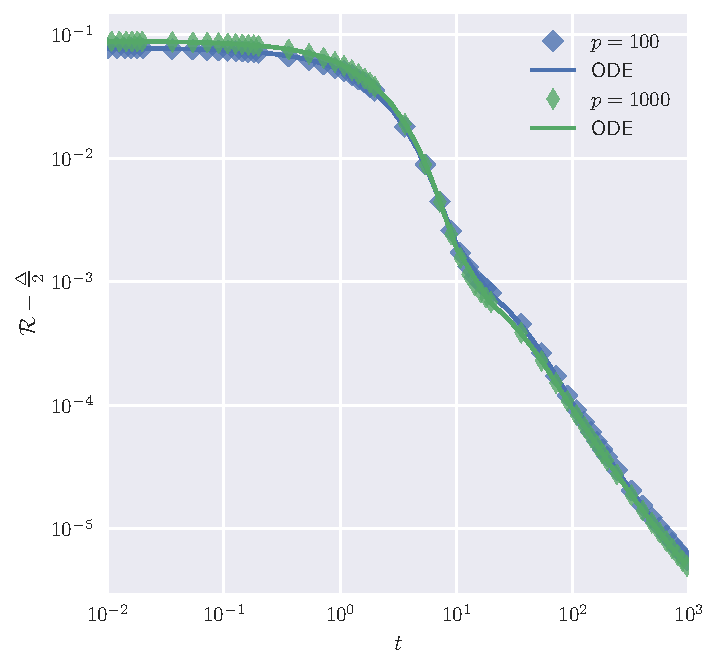
\includegraphics[width=\textwidth]{figs/mean-field/mf_limit_lowdim,fixedpoint_-k2_d5_activationerf_gamma1.0000_noise0.0}
        \begin{center}
            (a) \(\hidt=2,d=10,\lr=\num{1.},\noise=\num{0.},\sigma(x)=\erf(\sfrac{x}{\sqrt2})\)
        \end{center}
    \end{minipage}
    %
    \begin{minipage}[t]{.49\textwidth}
        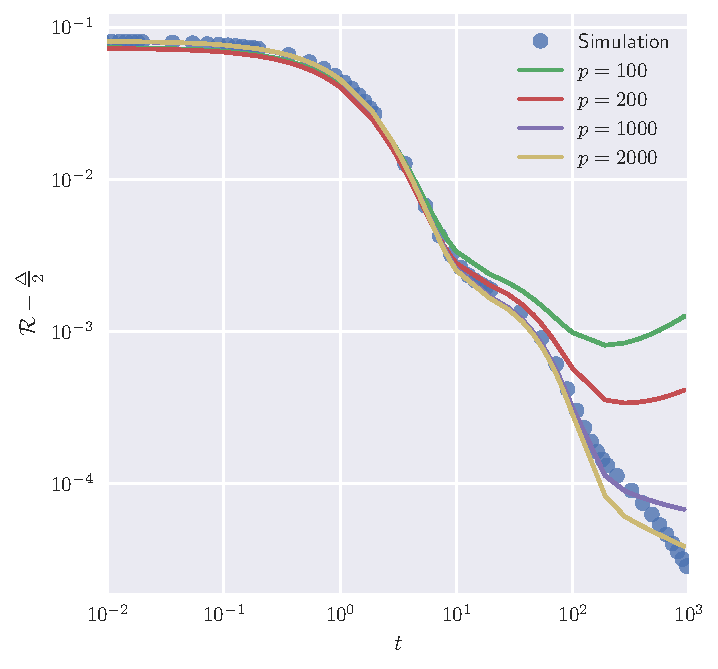
\includegraphics[width=\textwidth]{figs/mean-field/mf_limit_lowdim,onlydiag_-k2_d5_activationerf_gamma1.0000_noise0.0}
        \begin{center}
            (b) \(\hidt=2,d=5,\lr=\num{1.},\noise=\num{0.},\sigma(x)=\erf(\sfrac{x}{\sqrt2})\)
        \end{center}
    \end{minipage}
    %
    \begin{minipage}[t]{.49\textwidth}
        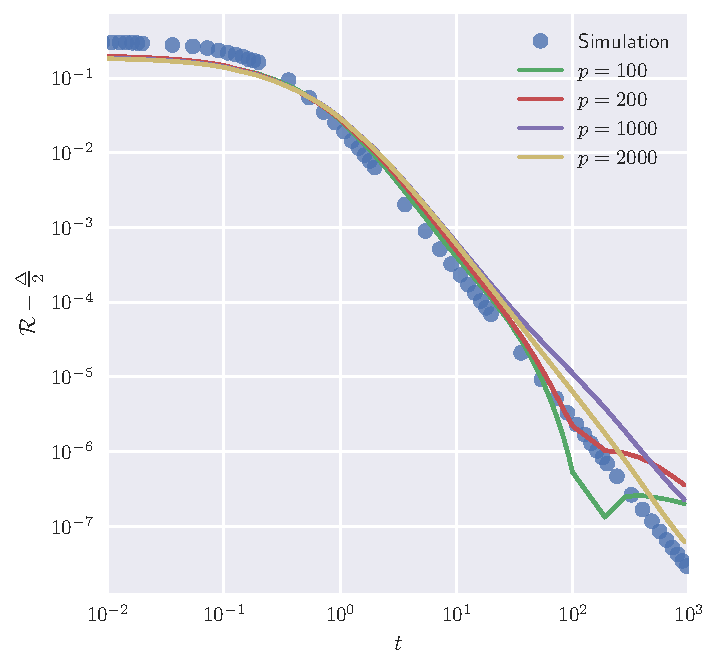
\includegraphics[width=\textwidth]{figs/mean-field/mf_limit_lowdim,onlydiag_-k2_d5_activationsquare_gamma1.0000_noise0.0}
        \begin{center}
            (c) \(\hidt=2,d=5,\lr=\num{1.},\noise=\num{0.},\sigma(x)=x^2\)
        \end{center}
    \end{minipage}
    %
    \begin{minipage}[t]{.49\textwidth}
        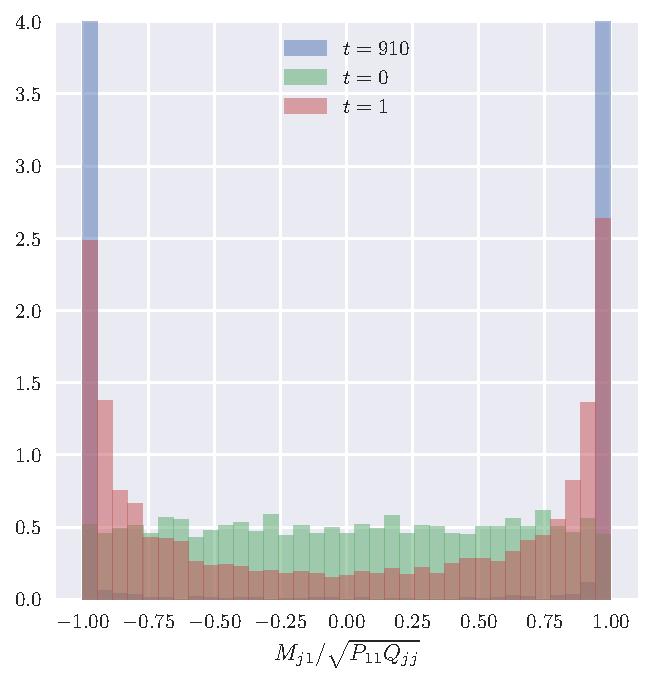
\includegraphics[width=\textwidth]{figs/mean-field/mf_limit_hist_-p5000_activationsquare_gamma1.0000_noise0.0}
        \begin{center}
            (d) \(\hidt=1,d=3,\lr=\num{1.},\noise=\num{0.},\sigma(x)=x^2\)
        \end{center}
    \end{minipage}

    \caption{
     (a) Evolution from starting point \(Q^\bot = 0\), tracking only \(\M\). (b) - (c)  Low-dimension simulations and the corresponding ODE trajectory, without the off-diagonal entries of matrix $\Xi$ (d) Histogram for the distribution of teacher student-teacher weights overlappings, at different times.
    }
    \label{2302:fig:mf-numerical-simulation-appendix}
\end{figure}
%%%%%%%%%%%%%%%%%%%%%%%%%%%%%%%%%%%%%%%%%%%%%%%%%%%%%%%%%%%%%%%%%%%%%%%%%%%%%%%
